\documentclass{article}
\usepackage{fontspec}

% Used to embed Sage code in latex
%\usepackage{sagetex}


% Math Environment
\usepackage{euler}        % Euler font
\usepackage{amsmath}      % Math macros
\usepackage{amssymb}      % Math symbols
\usepackage{unicode-math} % Unicode support

% Physics Environment
\usepackage{physics}


\usepackage[makeroom]{cancel} % Used to cancel terms in algebraic equations
\usepackage{ulem} % Different underline environments
\usepackage{polynom} %Polynomial long division

% Typesetting Rules
\setlength\parindent{0em}
\setlength\parskip{0.618em}
\usepackage[a4paper,lmargin=1in,rmargin=1in,tmargin=1in,bmargin=1in]{geometry}
\setmainfont[Mapping=tex-text]{Helvetica Neue LT Std 45 Light}

% Common Macros
\newcommand\N{\mathbb{N}}
\newcommand\Z{\mathbb{Z}}
\newcommand\Q{\mathbb{Q}}
\newcommand\R{\mathbb{R}}
\newcommand\C{\mathbb{C}}
\newcommand\A{\mathbb{A}}
\def\res{\mathop{\text{Res}}\limits}

% Color
\usepackage[dvipsnames]{xcolor}
\usepackage{pagecolor}
% \definecolor{DeepMossGreen}{HTML}{394820}
% \pagecolor{DeepMossGreen}
% \color{Goldenrod}

\usepackage{graphicx}

\begin{document}

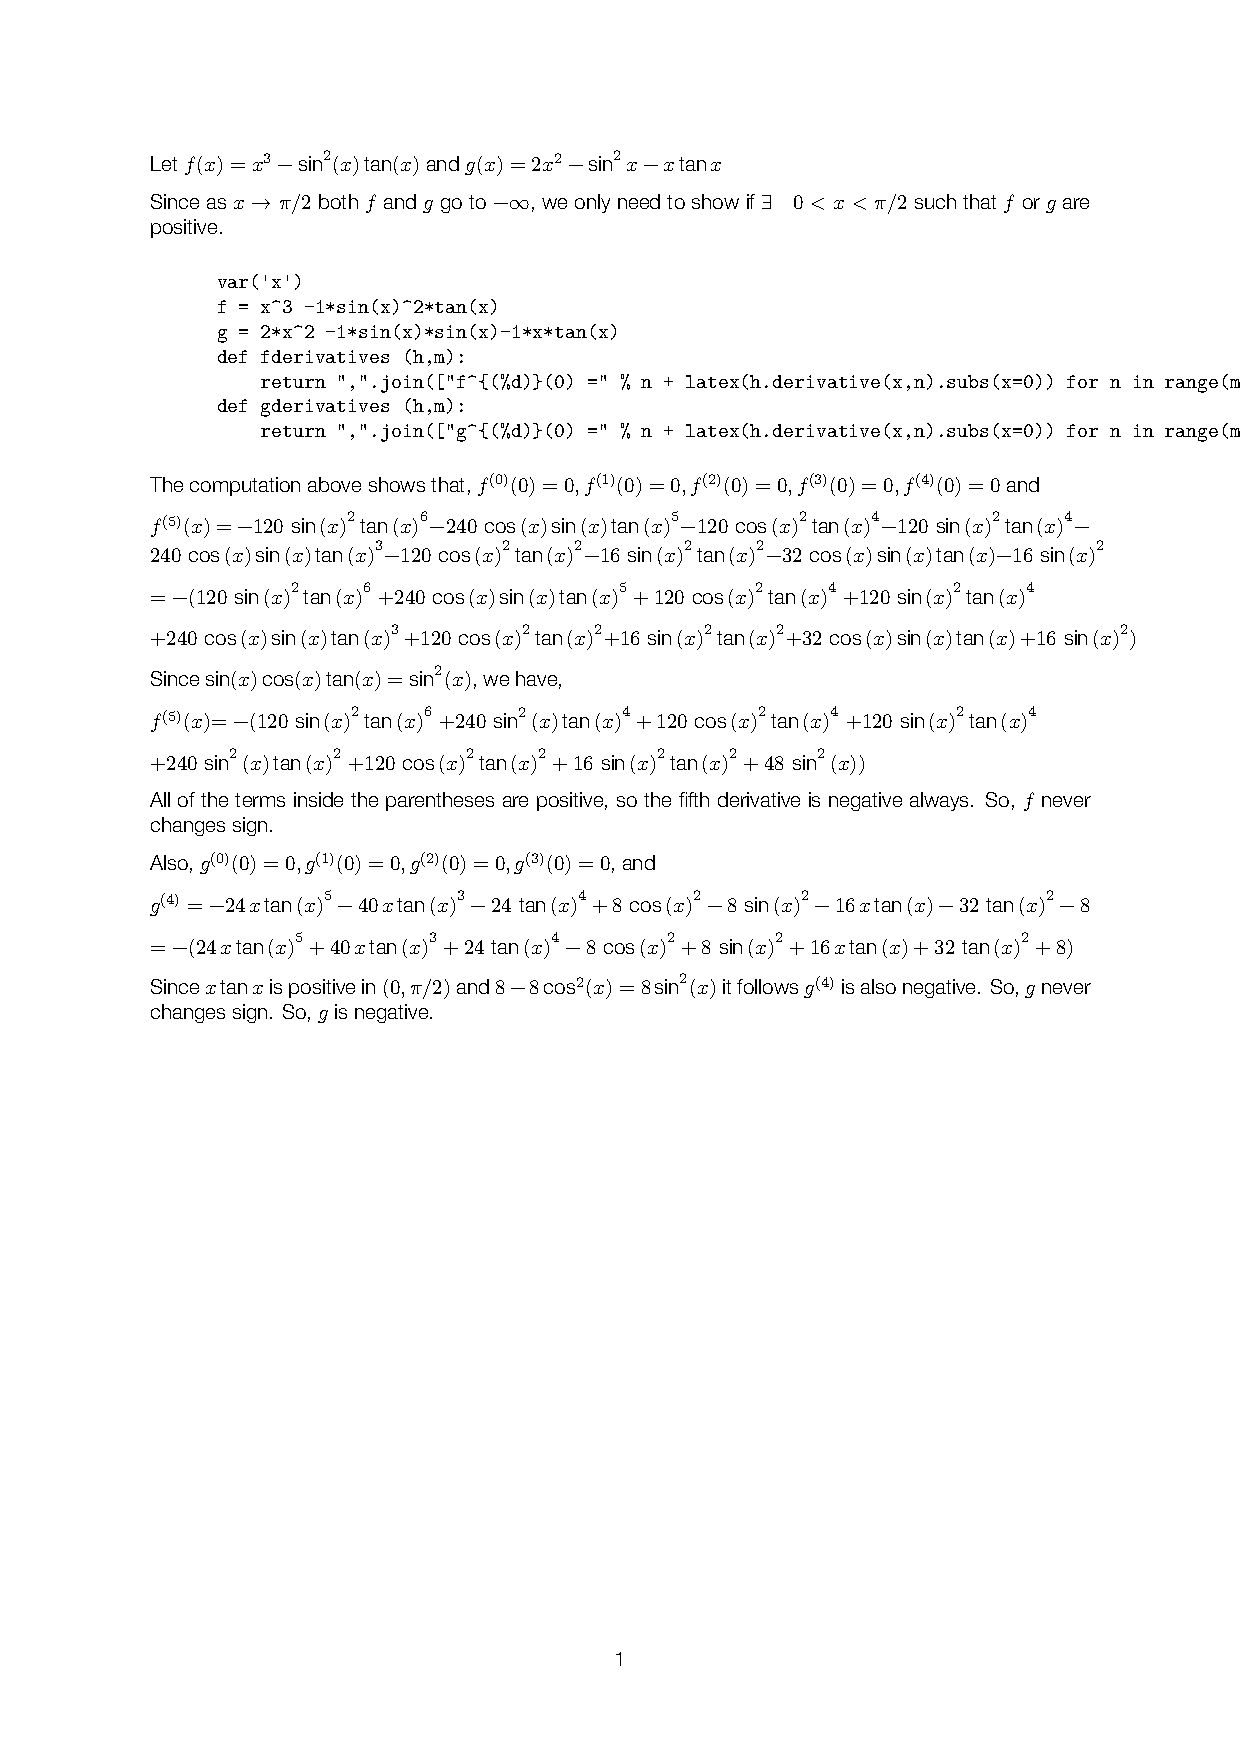
\includegraphics[width=\textwidth]{q2.png}

\uwave{slu.}

If $t\geq 0$, and $x = \sqrt{t}$, $\sqrt{t} = -\sqrt{t}+2\sqrt{t}$.

If $t\geq 0$, and $x = 2\sqrt{t}$, $0 = -2\sqrt{t}+2\sqrt{t}$.

If $t <0 $, and $-x = -\sqrt{|t|}$, $-\sqrt{|t|} =
\sqrt{|t|}-2\sqrt{|t|}$.

If $t < 0$, and $x = 2\sqrt{|t|}$, $0 = -2\sqrt{|t|}+2\sqrt{|t|}$.

Let $\varepsilon >0$, for $|t|<\varepsilon$, $|x|<\varepsilon$,
$|\phi(x,t)| < \sqrt{\varepsilon},$ as the maximum value of $\phi$ for
each $t$ is $\pm \sqrt{t}$.

So, $f$ is continuous at the origin because $\varepsilon$ was
arbitrary, and away from the origin all the pieces agree.

So, $f$ is
continuous on $\R^2$.

Since $\lim_{h\rightarrow 0} \frac{\sqrt{h}}{h} = \lim_{\rightarrow
  0}\frac{1}{\sqrt{h}} = 0$, we have both that,
\begin{align*}
 \lim_{h\rightarrow 0^+} \frac{\begin{cases}x & 0\leq x
      \leq \sqrt{h} \\ -x+2\sqrt{h} & \sqrt{h}\leq x \leq 2\sqrt{h}\\
      0 &\text{ otherwise}\end{cases} -\begin{cases}x & 0\leq x
      \leq \sqrt{0} \\ -x+2\sqrt{0} & \sqrt{0}\leq x \leq 2\sqrt{0}\\
      0 &\text{ otherwise}\end{cases}}{h}
               &= \lim_{h\rightarrow 0^+} \begin{cases}\frac{x}{h} & 0\leq x
      \leq \sqrt{h} \\ \frac{-x+2\sqrt{h}}{h} & \sqrt{h}\leq x \leq 2\sqrt{h}\\
      \frac{0}{h} &\text{ otherwise}\end{cases} = 0,
\end{align*}
and
\begin{align*}
 \lim_{h\rightarrow 0^-} \frac{\begin{cases}-x & 0\leq x
      \leq \sqrt{|h|} \\ x-2\sqrt{|h|} & \sqrt{|h|}\leq x \leq 2\sqrt{|h|}\\
      0 &\text{ otherwise}\end{cases}}{h}
               &= \lim_{h\rightarrow 0^-} \begin{cases}-\frac{x}{h} & 0\leq x
      \leq \sqrt{|h|} \\ \frac{x-2\sqrt{|h|}}{h} & \sqrt{|h|}\leq x \leq 2\sqrt{|h|}\\
      \frac{0}{h} &\text{ otherwise}\end{cases} = 0.
\end{align*}

So $\forall x\in \R, (D_2 f)(x,0) =0$.

By, the definition of $f(t)$ in the problem we have, for $1/4>t\geq 0$
\begin{align*}
  f(t) = \int_{-1}^{1}\phi(x,t) \dd{x}
  &= \int_0^1\phi(x,t)\dd{x}\\
  &= \int_0^{\sqrt{t}} x\dd{x} + \int_{\sqrt{t}}^{2\sqrt{t}}
    -x+2\sqrt{t}\dd{x}\\
  &= \frac{t}{2} +\left(  -\frac{x^2}{2}+2\sqrt{t}x\right) \bigg|_{\sqrt{t}}^{2\sqrt{t}}\\
  &= \frac{t}{2} -2t+4t +\frac{t}{2}-2t  = t.
\end{align*}

for, $-1/4<t \leq 0$ we have
\begin{align*}
  f(t) = \int_{-1}^{1}-\phi(x,|t|) \dd{x}
  &= \int_0^1-\phi(x,|t|)\dd{x}\\
  &= \int_0^{\sqrt{|t|}} -x\dd{x} +\int_{\sqrt{|t|}}^{2\sqrt{|t|}} x-2\sqrt{|t|}\dd{x}\\
  &= -\frac{|t|}{2} +\left(  \frac{x^2}{2}-2\sqrt{|t|}x\right) \bigg|_{\sqrt{|t|}}^{2\sqrt{|t|}}\\
  &= -\frac{|t|}{2} -2|t|+4|t| -\frac{|t|}{2}-2|t|  = -|t| = -(-t) = t.
\end{align*}

So, \[f'(t) = 1 \implies f'(0)= 1 \neq  0  = \int_{-1}^1 0\dd{x} =
  \int_{-1}^1 (D_2 \phi)(x,0) \dd{x}\quad \lozenge\]
\end{document}




%%% Local Variables:
%%% mode: latex
%%% TeX-master: t
%%% End:
